%&pdflatex
\documentclass[mathserif]{beamer} %, handout
\usetheme[progressbar=foot]{metropolis}
\setbeamertemplate{caption}[numbered]

\usepackage[utf8x]{inputenc}
\usepackage[T1]{fontenc}
\usepackage[english]{babel}

\usepackage{amssymb, amsmath, amsfonts, mathtools, mathrsfs}
\usepackage{changepage} % for alignwidth
\usepackage{tabu, tabulary}
\usepackage{comment}

\usepackage{tikz}
\usetikzlibrary{arrows,arrows.meta}

\AtBeginSubsection{
\frame[plain,c]{\subsectionpage}
}

\defbeamertemplate{subsection page}{simple}{
  \centering
  \usebeamercolor[fg]{subsection title}
  \usebeamerfont{subsection title}
  \insertsubsection\\
  \insertsubsectionhead\\
}
\setbeamertemplate{subsection page}[simple]

\title{Computational modeling of the Boltzmann equation: the projection-interpolation method and gas-kinetic unified algorithm}
\author[shortname]{
    \underline{Oleg Rogozin}\inst{1,2} \and
    Vladimir Aristov\inst{1} \and
    Ao-Ping Peng\inst{3,4} \and
    Zhi-Hui Li\inst{3,4}}
\institute[shortinst]{
    \inst{1} Dorodnicyn Computing Center of Russian Academy of Sciences, Russia \and
    \inst{2} Skolkovo Institute of Science and Technology, Russia \and
    \inst{3} Hypervelocity Aerodynamics Institute, CARDC, China \and
    \inst{4} National Laboratory for Computational Fluid Dynamics, China}
\date{}

\newcommand\pro{\item[$+$]}
\newcommand\con{\item[$-$]}

\newcommand{\Kn}{\mathrm{Kn}}
\newcommand{\Ma}{\mathrm{Ma}}
\newcommand{\dd}{\:\mathrm{d}}
\newcommand{\der}[2][]{\frac{\dd#1}{\dd#2}}
\newcommand{\derdual}[2][]{\frac{\dd^2#1}{\dd#2^2}}
\newcommand{\pder}[2][]{\frac{\partial#1}{\partial#2}}
\newcommand{\pderdual}[2][]{\frac{\partial^2#1}{\partial#2^2}}
\newcommand{\pderder}[2][]{\frac{\partial^2 #1}{\partial #2^2}}
\newcommand{\Pder}[2][]{\partial#1/\partial#2}
\newcommand{\dxi}{\boldsymbol{\dd\xi}}
\newcommand{\bxi}{\boldsymbol{\xi}}
\newcommand{\bh}{\boldsymbol{h}}
\newcommand{\be}{\boldsymbol{e}}
\newcommand{\Nu}{\mathcal{N}}
\newcommand{\OO}[1]{O(#1)}
\newcommand{\Set}[2]{\{\,{#1}:{#2}\,\}}
\newcommand{\deltann}[2]{(\delta_{#1#2}-n_#1 n_#2)}
\newcommand{\onwall}[1]{\left(#1\right)_0}
\newcommand{\xoverbrace}[2][\vphantom{\int}]{\overbrace{#1#2}}
\newcommand{\Cite}[2][]{\alert{\textsc{#2 #1}}}

\begin{document}

\frame{\titlepage}


\begin{frame}
  \frametitle{Plan}
  \linespread{0.8}
  \tableofcontents
\end{frame}

\section{Computational methods}

\subsection[]{Diversity \& History}

% balance between accuracy versatility of the numerical method
\begin{frame}
    \frametitle{Classical numerical methods for the Boltzmann equation}
    \centering
    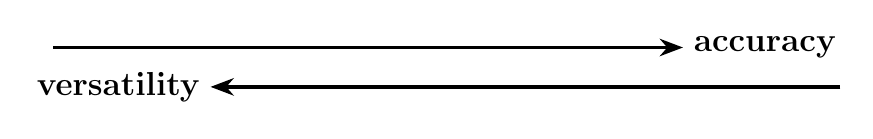
\begin{tikzpicture}
        \draw[very thick, -Stealth] (0,.5) -- (8,.5) node[right] {\bf\large \alert{accuracy}};
        \draw[very thick, -Stealth] (10,0)  -- (2,0) node[left] {\bf\large \alert{versatility}};
    \end{tikzpicture}

    \setlength{\leftmarginii}{10pt}
    \setlength{\leftmarginiii}{\leftmarginii}
    \begin{adjustwidth}{-2.5em}{-2.5em}
    \centering
    \begin{tabular}{p{0.35\textwidth}p{0.35\textwidth}p{0.35\textwidth}}
        % unbounded velocity space but low stochastic accuracy
		\centering\bfseries Statistical simulations &
		% conservative, second-order
		\centering\bfseries Discrete-velocity methods &
		% fast algorithms, spectral accuracy, Gibbs phenomenon, conservation and positivity issues
		{\centering\bfseries Projection methods (weighted residuals)} \\[10pt]
        Markov-type process reproducing Boltzmann dynamics &
		Fixed set of allowed molecular velocities &
		Expansion within some functional space \\
   		\begin{itemize}
            \item equal particles
            \item deviational, weighted
        \end{itemize} &
		\begin{itemize}
            \item discrete-gas models
            \item modification of the collision process
            \item stochastic acceleration
        \end{itemize} &
		\begin{itemize}
            \item Galerkin, collocation
            \item Hermite, Laguerre, Fourier, DG, wavelets, \dots
            \item Uncertainty quantification
        \end{itemize}
	\end{tabular}
    \end{adjustwidth}
\end{frame}

\begin{frame}
    \frametitle{Modification/mollification of the collision process}
    \centering
    {\Large\bf Discrete-velocity methods}\vspace{10pt}

    \Cite[1997]{Palczewski, Schneider, Bobylev}:\\ % Пальчевски, Шнайд'ер
        order of convergence < \(\frac14\) for discrete-velocity gas
    \vspace{10pt}
    \setlength{\leftmarginii}{10pt}
    \setlength{\leftmarginiii}{\leftmarginii}
    \begin{adjustwidth}{-2.5em}{-2.5em}
    \centering
    Computers \& Mathematics with Applications Vol. 35, No. 1-2\\
    (special issue edited by C.~Cercignani \& R.~Illner) % Рейнхард

    \newcommand{\ColW}{0.35\textwidth}
    \begin{tabular}{>{\centering\arraybackslash}p{\ColW}>{\centering\arraybackslash}p{\ColW}>{\centering\arraybackslash}p{\ColW}}
		\centering\bfseries Collisional integral &
		\centering\bfseries Collisional sphere &
		{\centering\bfseries Collisional pair} \\
		\Cite[1998]{Buet, Cordier, Degond} &
		\Cite[1998]{Babovsky}, \Cite{G\"orsch}

		\vspace{-10pt}
		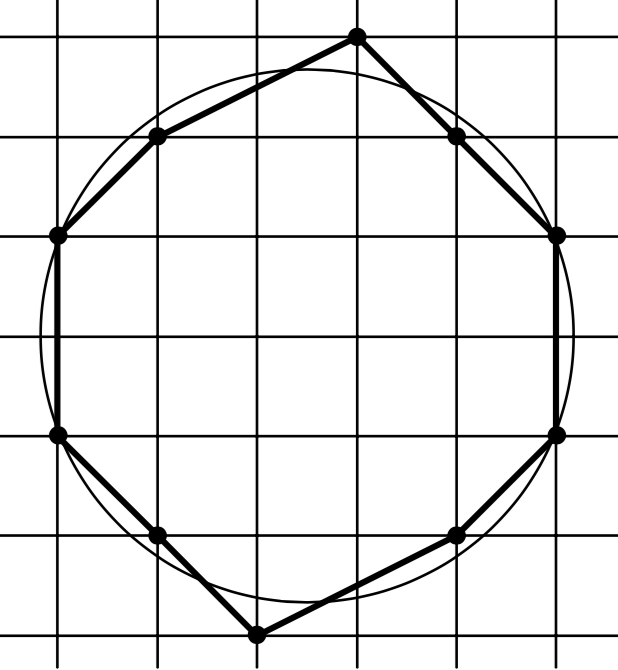
\includegraphics[width=2cm]{schemes/sphere} &
		\Cite[1998]{Tcheremissine}\vspace{5pt}
		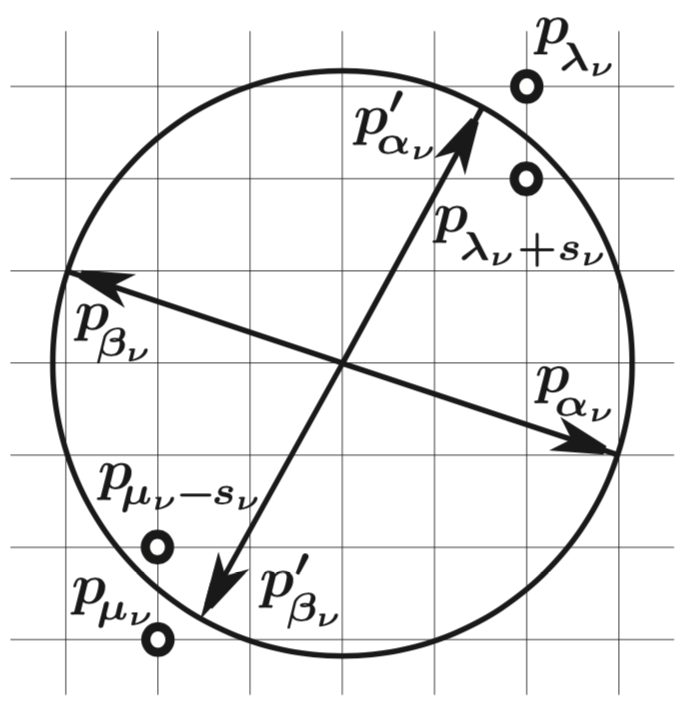
\includegraphics[width=2cm]{schemes/pair}
	\end{tabular}
    \end{adjustwidth}
\end{frame}

\subsection[(Tcheremissine's method)]
{Conservative and entropic second-order DVM}

\begin{frame}
    \frametitle{The discretization of the velocity space}
    Grid \(\mathcal{V} = \Set{\xi_\gamma}{\gamma\in\Gamma}\) is constructed so that
    \begin{equation}\label{eq:xi_cubature}
        \int F(\bxi) \dxi \approx \sum_{\gamma\in\Gamma} F_\gamma w_\gamma =
            \sum_{\gamma\in\Gamma} \hat{F_\gamma},
            \quad F_\gamma = F(\bxi_\gamma),
    \end{equation}\vspace{-10pt}

    where \(\sum_{\gamma\in\Gamma} w_\gamma = V_\Gamma\) is the volume of the velocity grid.
    \pause\vspace{20pt}

    The symmetrized collision integral\vspace{-20pt}

    \begin{equation}\label{eq:symm_ci}
        J(f_\gamma, f_\gamma) = \frac14\int \left(
            \delta_\gamma + \delta_{\gamma*} - \delta'_\gamma - \delta'_{\gamma*}
        \right) (f'f'_* - ff_*)B \dd\Omega(\boldsymbol{\alpha}) \dxi\dxi_*
    \end{equation}\vspace{-30pt}

    has the following discrete analogue: % quantities with accents
    \begin{equation}\label{eq:discrete_symm_ci}
        \footnotesize
        \hat{J}_\gamma = \frac{\pi V_\Gamma^2}{\displaystyle\sum_{\nu\in\Nu} w_{\alpha}w_{\beta}}
            \sum_{\nu\in\Nu} \bigg(
                \delta_{\alpha\gamma} + \delta_{\beta\gamma} -
                \xoverbrace{ \alert{\delta_{\alpha'\gamma}} - \alert{\delta_{\beta'\gamma}} }^\text{projection}
            \bigg)\bigg(
                \xoverbrace{ \frac{w_{\alpha}w_{\beta}}{\alert{w_{\alpha'}w_{\beta'}}}
                \alert{\hat{f}_{\alpha'}\hat{f}_{\beta'}} }^\text{interpolation} - \hat{f}_{\alpha}\hat{f}_{\beta}
            \bigg)B_\nu.
    \end{equation}\vspace{-10pt}
\end{frame}

\begin{frame}
    \frametitle{Conservative projection}
    \centering{\Large\bf Why the method is called as "projection"?} % why, actually, ...
    \vspace{10pt}

    Petrov--Galerkin projection method:
    \begin{equation}\label{eq:Petrov-Galerkin}
        \int \xoverbrace{ \psi_s(\bxi_\gamma) }^\text{test space} \bigg(
            \alert{\delta(\bxi'-\bxi_\gamma)} - \sum_{a\in\Lambda} r_{\lambda,a}
            \xoverbrace{ \delta(\bxi_{\lambda+s_a}-\bxi_\gamma) }^\text{trial space}
        \bigg) \dxi_\gamma = 0.
    \end{equation}
    \begin{itemize}
        \item \(r_{\lambda,a}\) are the \emph{projection weights} (in space \(\mathcal{V}\))
        \item \(\mathcal{S} = \Set{s_a}{a\in\Lambda, r_{\lambda,a}\neq0}\) is the \emph{projection stencil}
            \\ (set of displacement rules)
        \item \(\psi_0 = 1, \psi_i = \xi_i, \psi_4 = \xi_i^2\) are the \emph{collisional invariants}
        \item the same holds for \(\alert{\delta(\bxi'_*-\bxi_\gamma)}\)
    \end{itemize}
\end{frame}

\begin{frame}
    \frametitle{Interpolation of the distribution function}
    As a general example, use the weighted Kolmogorov mean: % we have many freedom to define the interpolation procedure
    \begin{equation}\label{eq:Kolmogorov_mean}
        \begin{dcases}
            \alert{\hat{f}_{\alpha'}} = \phi^{-1}_f\left(\sum_{a\in\Lambda} q_{\lambda,a}
                \phi_f\left(\hat{f}_{\lambda+s_a}\right)\right), \\
            \alert{w_{\alpha'}} = \phi^{-1}_w\left(\sum_{a\in\Lambda} p_{\lambda,a}
                \phi_w\left(w_{\lambda+s_a}\right)\right), \\
        \end{dcases}
    \end{equation}
    If we take the geometric mean
    \begin{equation}\label{eq:geometric_mean}
       \phi_{f,w}(x) = \ln(x), \quad \phi_{f,w}^{-1}(x) = \exp(x), \quad p_{\lambda,a} = q_{\lambda,a} = r_{\lambda,a},
    \end{equation}
    then \(\mathcal{H}\)-theorem holds and
    \begin{equation}\label{eq:strict_interpolation}
        \hat{J}_\gamma(\hat{f}_{M\gamma}, \hat{f}_{M\gamma}) = 0.
    \end{equation}
    The same should hold for \(\alert{w_{\beta'}}\) and \(\alert{\hat{f}_{\beta'}}\).
\end{frame}

\begin{frame}
    \frametitle{Cauchy problem for the space-homogeneous BE}
    Rewrite
    \begin{equation}
        \hat{J}_\gamma = \frac{\pi V_\Gamma^2}{\sum_{\nu\in\Nu} w_{\alpha}w_{\beta}}
        \sum_{\nu\in\Nu} \left(
            \delta_{\alpha\gamma} + \delta_{\beta\gamma} -
            \delta_{\alpha'\gamma} - \delta_{\beta'\gamma}
        \right)\big(\cdots\big)B_\nu
    \end{equation}
    as
    \begin{equation}
        \hat{J}_{\gamma} = \sum_{j=1}^N \hat{\Delta}_{\gamma}^{n+(j-1)/N}, \quad N=|\Nu|.
    \end{equation}
    Then we can build a conservative scheme in fractional steps
    \begin{equation}\label{eq:fractional_step_scheme}
        \hat{f}_\gamma^{n+j/N} = \hat{f}_\gamma^{n+(j-1)/N} + \frac{t_{n+1}-t_n}{N}\hat{\Delta}_{\gamma}^{n+(j-1)/N}
        \quad (j = 1,\dotsc,N).
    \end{equation}
    \pause
    \begin{itemize}
        \item every \(\hat{\Delta}_{\gamma}^{n+(j-1)/N}\) contains \(2(1+|\mathcal{S}|)\) nonzero elements
        \item every fractional step preserve mass, momentum, energy and does not decrease entropy!
    \end{itemize}
\end{frame}

\begin{frame}
    \frametitle{Positivity of the distribution function}
    To ensure positivity in practice, some cubature points (say, \(\mathcal{M}\)) can be excluded:
    \begin{equation}\label{eq:discrete_short_ci_discarded}
        \hat{J}_\gamma = \sum_{\nu\in\Nu\alert{\setminus\mathcal{M}}} \hat{\Delta}_{\gamma\nu}.
    \end{equation}
    \vspace{10pt}

    \(|\Nu|\) is adapted to control a smallness of the excluded-points contribution in each physical cell:
    \begin{equation}\label{eq:excluded_contribution}
        \frac{\sum_{\nu\in\mathcal{M}} \left| \hat{\Delta}_{\alpha\nu} \right|}
            {\sum_{\nu\in\Nu\setminus\mathcal{M}} \left| \hat{\Delta}_{\alpha\nu} \right|} < \varepsilon.
    \end{equation}
    Usually, \(\varepsilon \lesssim 10^{-5}\) for high-accuracy solution.
\end{frame}

\subsection[]{Gas-kinetic unified algorithm (GKUA)}

\begin{frame}
    \frametitle{Theoretical comparison}
    \begin{columns}[T]
        \begin{column}{6cm}
            \begin{block}{\centering \underline{Tcheremissine's method}}
                Suitable for high-accuracy solution of boundary-value problems
                \begin{itemize}
                    \item original Boltzmann equation
                    \item conservative, entropic, positive
                    \item explicit scheme
                \end{itemize}
            \end{block}
        \end{column}
        \begin{column}{6cm}
            \begin{block}{\centering \underline{Gas-Kinetic Unified Algorithm}}
                Suitable for high-speed engineering applications
                \begin{itemize}
                    \item Shakhov model
                    \item FD scheme without correction
                    \item implicit scheme
                \end{itemize}
            \end{block}
        \end{column}
    \end{columns}
\end{frame}

\section{Numerical results}

\subsection[]{Cylinder at 90 km altitude}

\begin{frame}
    \frametitle{Cylinder, 90 km, \(\Ma=2.4\), \(\Kn=0.13\), \(T_\mathrm{body}=2.9\), VHS}
    \begin{center}
        \includegraphics[width=0.9\linewidth, clip=true, trim = 90 30 75 50 mm]%
            {cylinder-90km/mach-dsmc}
    \end{center}
\end{frame}

\begin{frame}
    \frametitle{Close-up of the Mach number contours}
    \begin{center}
        \includegraphics[width=\textwidth, clip=true, trim = 260 260 410 270 mm]%
            {cylinder-90km/mach-dsmc}
    \end{center}
\end{frame}

\begin{frame}
    \frametitle{Cylinder, 90 km, \(\Ma=2.4\), \(\Kn=0.13\), \(T_\mathrm{body}=2.9\), VHS}
    \begin{center}
        \includegraphics[width=0.9\linewidth, clip=true, trim = 90 30 75 50 mm]%
            {cylinder-90km/mach-gkua}
    \end{center}
\end{frame}

\begin{frame}
    \frametitle{Close-up of the Mach number contours}
    \begin{center}
        \includegraphics[width=\textwidth, clip=true, trim = 260 260 410 270 mm]%
            {cylinder-90km/mach-gkua}
    \end{center}
\end{frame}

\begin{frame}
    \frametitle{Temperature in the wake region}
    \begin{center}
        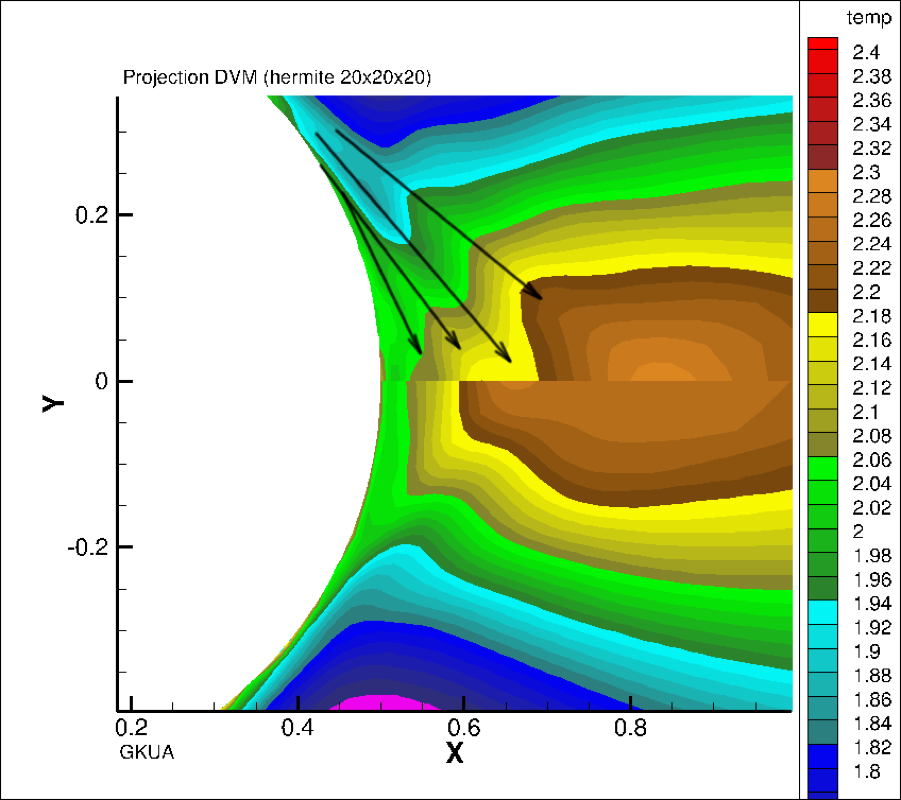
\includegraphics[width=0.5\textwidth]{cylinder-90km/temp-crude}
        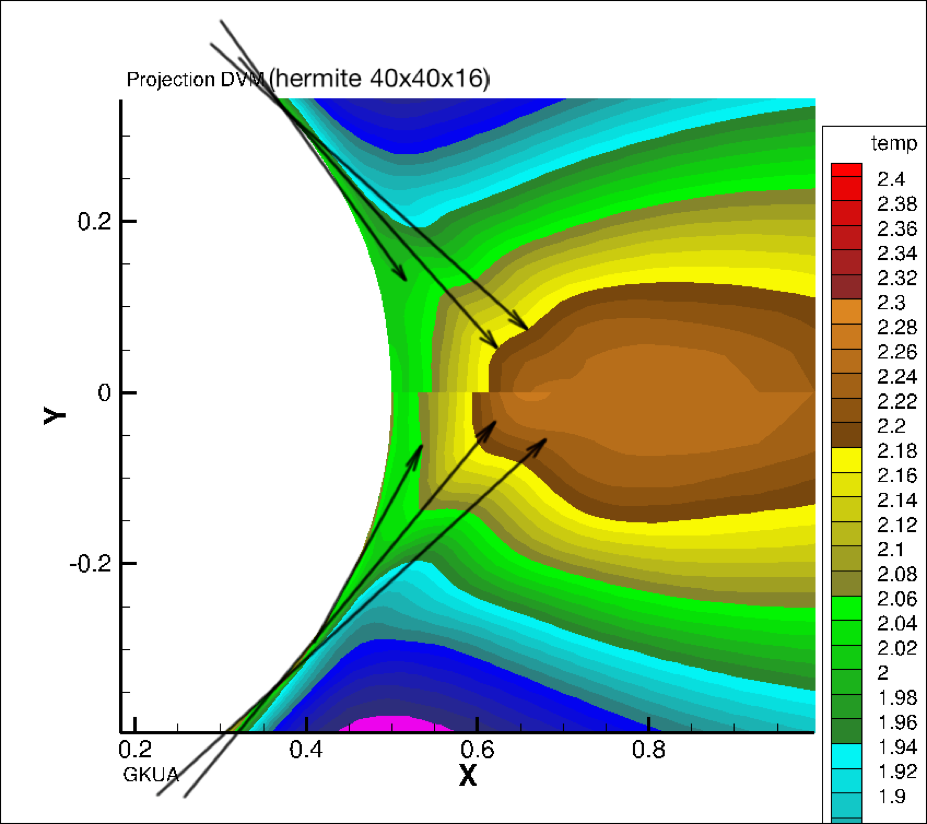
\includegraphics[width=0.5\textwidth]{cylinder-90km/temp-fine}
    \end{center}
\end{frame}

\subsection[]{Cylinder at 70 km altitude}

\begin{frame}
    \frametitle{Cylinder, 70 km, \(\Ma=3.0\), \(\Kn=0.0055\), \(T_\mathrm{body}=4.06\), VHS}
    \begin{center}
        \includegraphics[width=0.9\linewidth, clip=true, trim = 90 30 75 50 mm]%
            {cylinder-70km/mach-gkua}
    \end{center}
\end{frame}

\begin{frame}
    \frametitle{Close-up of the Mach number contours}
    \begin{center}
        \includegraphics[width=\textwidth, clip=true, trim = 200 260 470 270 mm]%
            {cylinder-70km/mach-gkua}
    \end{center}
\end{frame}

\begin{frame}
    \frametitle{Cylinder, 70 km, \(\Ma=3.0\), \(\Kn=0.0055\), \(T_\mathrm{body}=4.06\), VHS}
    \begin{center}
        \includegraphics[width=0.9\linewidth, clip=true, trim = 90 30 75 50 mm]%
            {cylinder-70km/uz-gkua}
    \end{center}
\end{frame}

\begin{frame}
    \frametitle{Close-up of the \(U_z\) contours}
    \begin{center}
        \includegraphics[width=\textwidth, clip=true, trim = 180 260 470 270 mm]%
            {cylinder-70km/uz-gkua}
    \end{center}
\end{frame}

\section{Conclusions}

\begin{frame}
    \frametitle{Concluding remarks}
    \begin{itemize}
        \item Stochastic techniques improve deterministic methods.
        \item Conservation properties are important in general case, especially for crude meshes.
        \item Lack of conservation properties is not the issue for external flows.
        \item Ray effect can distort solution in the wake zone.
    \end{itemize}
\end{frame}

%%%%%%%%%%%%%%%%%%%%%%%%%%%%%%%%%%%%%%%%%%%%%%%%%%%%%%%%%%%%%%%%%%%%%%%%%%%%%%%%%%%%%%%%%%
%%%                 To the memory of M. Kogan and O. Friedlander                       %%%
%%%%%%%%%%%%%%%%%%%%%%%%%%%%%%%%%%%%%%%%%%%%%%%%%%%%%%%%%%%%%%%%%%%%%%%%%%%%%%%%%%%%%%%%%%

\begin{frame}
    \frametitle{Slightly rarefied flows for \(\Ma=\OO{\Kn}\) and \(T=\OO{1}\)}
	\centering
    Zhukovsky, Moscow region\\
	{\Large\bf Central Aerohydrodynamics Institute \\ (TsAGI)}
    \vspace{20pt}

    \begin{columns}
		\column{.35\textwidth}\centering
		\textbf{Mikhail N. Kogan} \\ (1925 -- 2011) \\\vspace{5pt}
		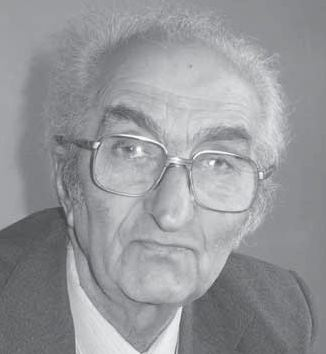
\includegraphics[height=3cm]{photos/Kogan}
		\column{.35\textwidth}\centering
		\textbf{Vladlen S. Galkin} \\ (born in 1932) \\\vspace{5pt}
		\vspace{3cm}
		\column{.35\textwidth}\centering
		\textbf{Oscar G. Friedlander} \\ (1939 -- 2015) \\\vspace{5pt}
		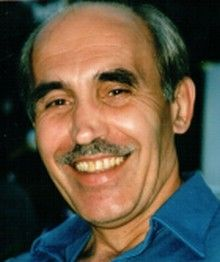
\includegraphics[height=3cm]{photos/Friedlander}
	\end{columns}
\end{frame}

\begin{frame}
    \frametitle{Slightly rarefied flows for \(\Ma=\OO{\Kn}\) and \(T=\OO{1}\)}
    \Cite[1976]{Kogan, Galkin, Friedlander} (notation follows \Cite[2007]{Sone})
    \begin{align*}
        \pder{x_i}\left(\frac{u_{i1}}{T_0}\right) &= 0, \\
        \pder{x_j}\left(\frac{u_{i1}u_{j1}}{T_0}\right)
            &-\frac12\pder{x_j}\left[\Gamma_1\left(
                \pder[u_{i1}]{x_j} + \pder[u_{j1}]{x_i} - \frac23\pder[u_{k1}]{x_k}\delta_{ij}
            \right)\right] \\
            &-\alert{\left[
                \frac{\Gamma_7}{\Gamma_2}\frac{u_{j1}}{T_0}\pder[T_0]{x_j}
                + \frac{\Gamma_2^2}4 \der{T_0}\left(\frac{\Gamma_7}{\Gamma_2^2}\right)
                    \left(\pder[T_0]{x_j}\right)^2
            \right]\pder[T_0]{x_i}} \\
            &= -\frac12\pder[p_0^\dag]{x_i}, \\
        \pder[u_{i1}]{x_i} &= \frac12\pder{x_i}\left(\Gamma_2\pder[T_0]{x_i}\right),
    \end{align*}
    where
    \begin{equation*}
    p_0^\dag = p_0 p_0
        + \frac23\pder{x_k}\left(\alert{\Gamma_3}\pder[T_0]{x_k}\right)
        - \frac{\alert{\Gamma_7}}{6}\left(\pder[T_0]{x_k}\right)^2, \quad u_{i1} = p_0v_{i1}.
    \end{equation*}
\end{frame}

\begin{frame}
    \frametitle{Kogan--Galkin--Friedlander equations}
    \centering{\Large\bf How to call them?}
    \begin{itemize}
        \item SNIF equations \Cite[1993]{Kogan}, \Cite[1995]{Bobylev}
        \item ghost effect equations \Cite[2009]{Levermore+}, \Cite[2017]{Aoki+}
        \item Kogan--Galkin--Friedlander equations \Cite[2017]{Rogozin}
    \end{itemize}
    \vspace{10pt}

    \centering{\Large\bf Experimental evidence}
    \begin{itemize}
        \item \Cite[1997, 2003]{Friedlander, Nikolsky et al.}:\\
            in low-density wind tunnels (TsAGI)
    \end{itemize}
\end{frame}

\begin{frame}
    \frametitle{The velocity field for \(\Kn=0.02\), \(T_1/T_0=5\) [Rogozin 2017]}
    \vspace{-10pt}
    \begin{figure}
        \footnotesize
        \hspace{-.5cm}
        \begin{overprint}
            \onslide<1| handout:3>
                \vspace{-5pt}
                \Cite[1998]{Aoki, Sone, Waniguchi} studied the problem by DSMC for \(0.1 \leq \Kn \leq 5\).
                \vspace{-5pt}

                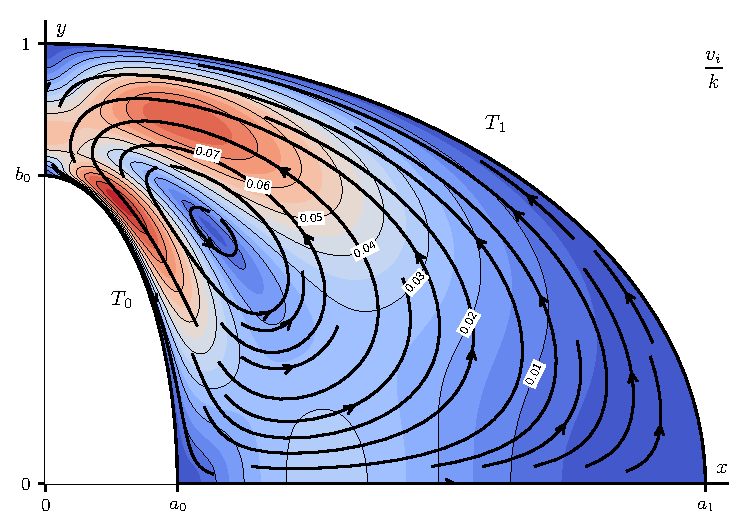
\includegraphics[width=\linewidth]{{{elliptic/kgf-0.02-flow}}}
                \vspace{-15pt}
                \caption{The KGF equations with the \alert{leading}-order boundary conditions}
            \onslide<2| handout:2>
                \vspace{-5pt}
                BC and Knudsen-layer correction are due to \Cite[1989]{Ohwada, Sone, Aoki}
                \vspace{-5pt}

                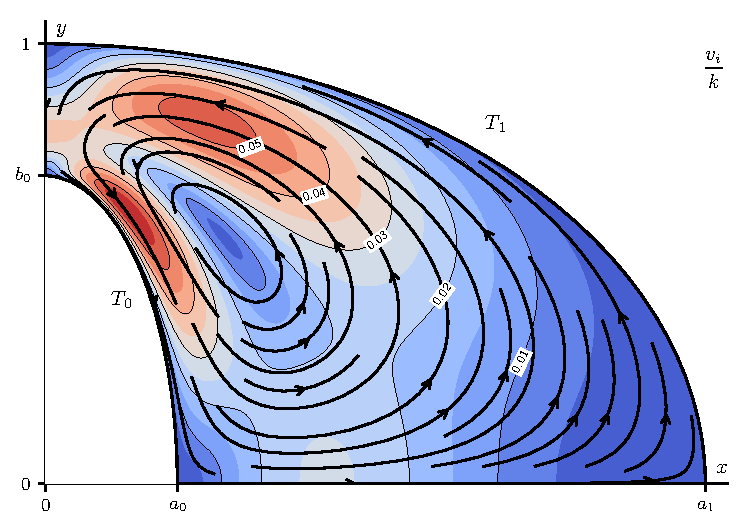
\includegraphics[width=\linewidth]{{{elliptic/first-0.02-flow}}}
                \vspace{-15pt}
                \caption{The KGF equations with the \alert{first}-order boundary conditions}
            \onslide<3| handout:1>
                \vspace{-5pt}
                BC and Knudsen-layer correction are due to \Cite[2015]{Takata, Hattori}
                \vspace{-5pt}

                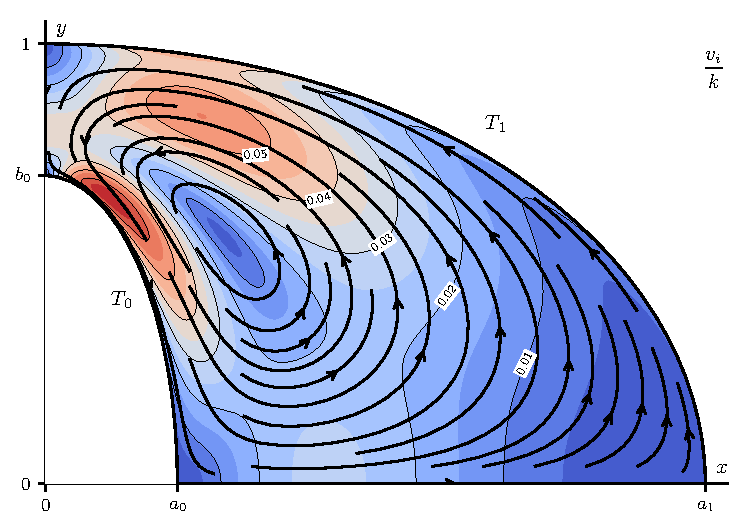
\includegraphics[width=\linewidth]{{{elliptic/second-0.02-flow}}}
                \vspace{-15pt}
                \caption{The KGF equations with the \alert{second}-order boundary conditions\!\!\!\!\!\!\!\!\!}
            \onslide<4| handout:0>
                \vspace{-5pt}
                Nonuniform velocity grid helps to approximate gas for \(1\leq T\leq5\).
                \vspace{-5pt}

                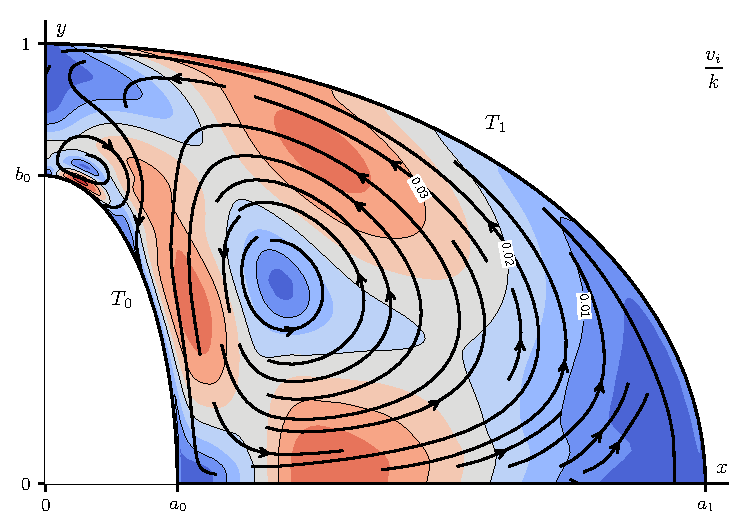
\includegraphics[width=\linewidth]{{{elliptic/kes-0.02-flow}}}
                \vspace{-15pt}
                \caption{Numerical solution of the Boltzmann equation}
        \end{overprint}
    \end{figure}
\end{frame}

\begin{frame}
    \frametitle{}
    \centering
    \huge\bf Thank you!
\end{frame}

\end{document}
